\documentclass[12pt]{article}

\usepackage{assets/helpers/sbc-template}
\usepackage{graphicx,url}
\usepackage{algorithm}
\usepackage{algorithmic}
\usepackage[brazil]{babel}   
\usepackage[utf8]{inputenc}  

\floatname{algorithm}{Algoritmo}

\sloppy

\title{Desenvolvimento de um dispositivo IoT para monitoramento em tempo real de umidade e temperatura de um home office}

\author{Isabella de Freitas Nunes\inst{1}}

\address{Universidade do Vale do Itajaí
  (Univali)\\
  Rua Uruguai, 458 - Centro - Itajaí - Santa Catarina - Brasil - 88302-901
  \email{isabella.nunes@edu.univali.br}
}

\begin{document} 

\maketitle

\begin{abstract}
  This report describes a project of an IoT system implemented using an ESP8266 microcontroller with FreeRTOS framework. The system uses a DHT11 sensor for temperature and humidity monitoring, then MQTT protocol is used to transmit collected data to a broker. The solution includes Wi-Fi management, real-time status monitoring, and fault tolerance to maintain reliability in data acquisition and transmission. Also a local Frontend was developed using React, to use the data sent to the broker and monitor a home office.
\end{abstract}
     
\begin{resumo} 
  Este relatório descreve um projeto de um sistema de IoT implementado utilizando o microcontrolador ESP8266 com o framework FreeRTOS. O sistema usa um sensor DHT11 para monitoramento de temperatura e umidade e, em seguida, o protocolo MQTT é usado para transmitir os dados coletados a um broker. A solução inclui gerenciamento de Wi-Fi, monitoramento de status em tempo real e tolerância a falhas para manter a confiabilidade na aquisição e transmissão de dados. Também foi desenvolvido um Frontend local utilizando React, para utilizar os dados enviados ao broker e monitorar um home office.
\end{resumo}

\section{Introdução}

Nos últimos anos, a Internet das Coisas (IoT) tornou-se uma das tecnologias mais importantes e em crescente utilização por todo o mundo. A possibilidade de conectar objetos do cotidiano - eletrodomésticos, carros, termostatos, babás eletrônicas - à Internet por meio de dispositivos embarcados, possibilitou uma comunicação contínua entre pessoas, processos e coisas.

Por meio da computação de baixo custo, da nuvem, do big data, da análise de dados e das tecnologias móveis, agora é possível que objetos compartilhem e coletem dados com o mínimo de intervenção humana. Algo que no passado, motivou a criação de linguagens de programação como Java e que existiam apenas no imaginário dos pesquisadores.

Atualmente o mundo está se adaptando ao protocolo IPV6, onde é dito como metáfora, que será possível atribuir um endereço IP para cada grão de areia da terra. Com alta disponibilidade de conexão e os sistemas sendo capazes de registrar, monitorar e ajustar cada interação com as necessidades do sujeito ao seu redor, o mundo físico encontra o mundo digital e eles interagem entre si.

\section{Problema}

Considerando que esse relatório é referente a disciplina de Internet das Coisas, do Programa de Mestrado em Computação Aplicada da Universidade do Vale do Itajaí. Faz-se necessário que algumas aplicações práticas sejam desenvolvidas, a fim de que o conteúdo da disciplina seja melhor internalizado.

Portanto, o problema a ser explorado nesse relatório, consiste em realizar a implementação de um sistema de monitoramento utilizando um microcontrolador ESP8266 e um sensor de temperatura e umidade DHT11, fornecidos pelo programa. Além da implementação local, é necessário que o sistema faça a coleta e a transmissão dos dados em tempo real para um broker MQTT, possibilitando sua integração com plataformas como o Node-RED. A fim de que um dashboard seja construído, contendo as diferentes temperaturas e umidades do home office de todos os alunos, que estão geograficamente distribuídos.

\section{Objetivo}

O objetivo deste relatório é demonstrar como se deu o desenvolvimento da solução para o problema apresentado no capítulo 2. Ou seja, desenvolver um sistema IoT funcional que integra hardware e software para monitorar dados do home office do aluno, e enviá-los utilizando o protocolo MQTT. 

\section{Hardware}

Neste capítulo, as especificações técnicas dos componentes e como eles foram utilizados no projeto desenvolvido, serão descritas, bem como suas configurações, desafios, entre outros.
\subsection{ESP8266}

O ESP8266 é um microcontrolador com Wi-Fi de baixo custo desenvolvido pela Espressif Systems. Com esse dispositivo, é possível controlar entradas e saídas como se faz com um Arduino, entretanto sem adicionar um módulo de conexão Wireless, visto que ele já possuí um adaptador embutido. Ele se destaca por fornecer:

\begin{itemize}
  \item Baixo custo
  \item Baixo consumo de energia
  \item Conectividade
  \item Compatibilidade com diversas tecnologias
\end{itemize}

Segundo o manual técnico do fabricante, ele possuí um processador RISC L106 de 32 bits rodando a 80 ou 160 MHz, 32 KiB de RAM de instrução, Wi-Fi IEEE 802.11 b/g/n com suporte a autenticação WEP ou WPA/WPA2 ou redes abertas e 17 pinos GPIO para conexões diversas.

\subsection{DHT11}

O DHT11 é um sensor utilizado para medir temperatura e umidade relativa do ambiente. Esse sensor usa uma câmara de calibração para suas leituras e o coeficiente dessa calibração é salvo em uma memória OTP. Quando solicitado, o sensor entrega o coeficiente que está armazenado em sua memória. É um dispositivo pequeno, barato, que fornece baixo consumo e longa distância de transmissão (100m).

\subsection{Esquema de Conexão}

A imagem a seguir, demonstra como foi o planejamento de conexão dos dispositivos e suas ligações no microcontrolador. 

\begin{figure}[ht]
  \centering
  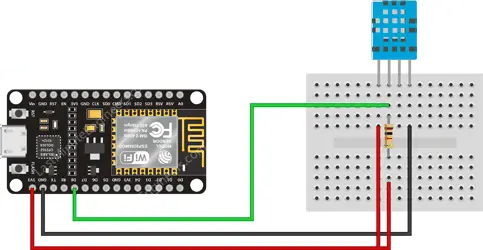
\includegraphics[width=.6\textwidth]{assets/img/schema.png}
  \caption{Projeto de conexão dos dispositivos}
\end{figure}

O DHT11 foi conectado ao ESP8266 utilizando o GPIO4, que é indicado para esse tipo de sensor. Um resistor de pull-up de 10 Kilo ohms foi conectado entre o pino de dados e o pino VCC do sensor, a fim de estabilizar o sinal. 

Um dos pinos 3.3V está conectado à linha de alimentação do sensor de temperatura e também de sua saída de dados. Bem como o pino GND está conectado à linha negativa do sensor, servindo como terra. A próxima imagem é do projeto após a montagem.

\begin{figure}[ht]
  \centering
  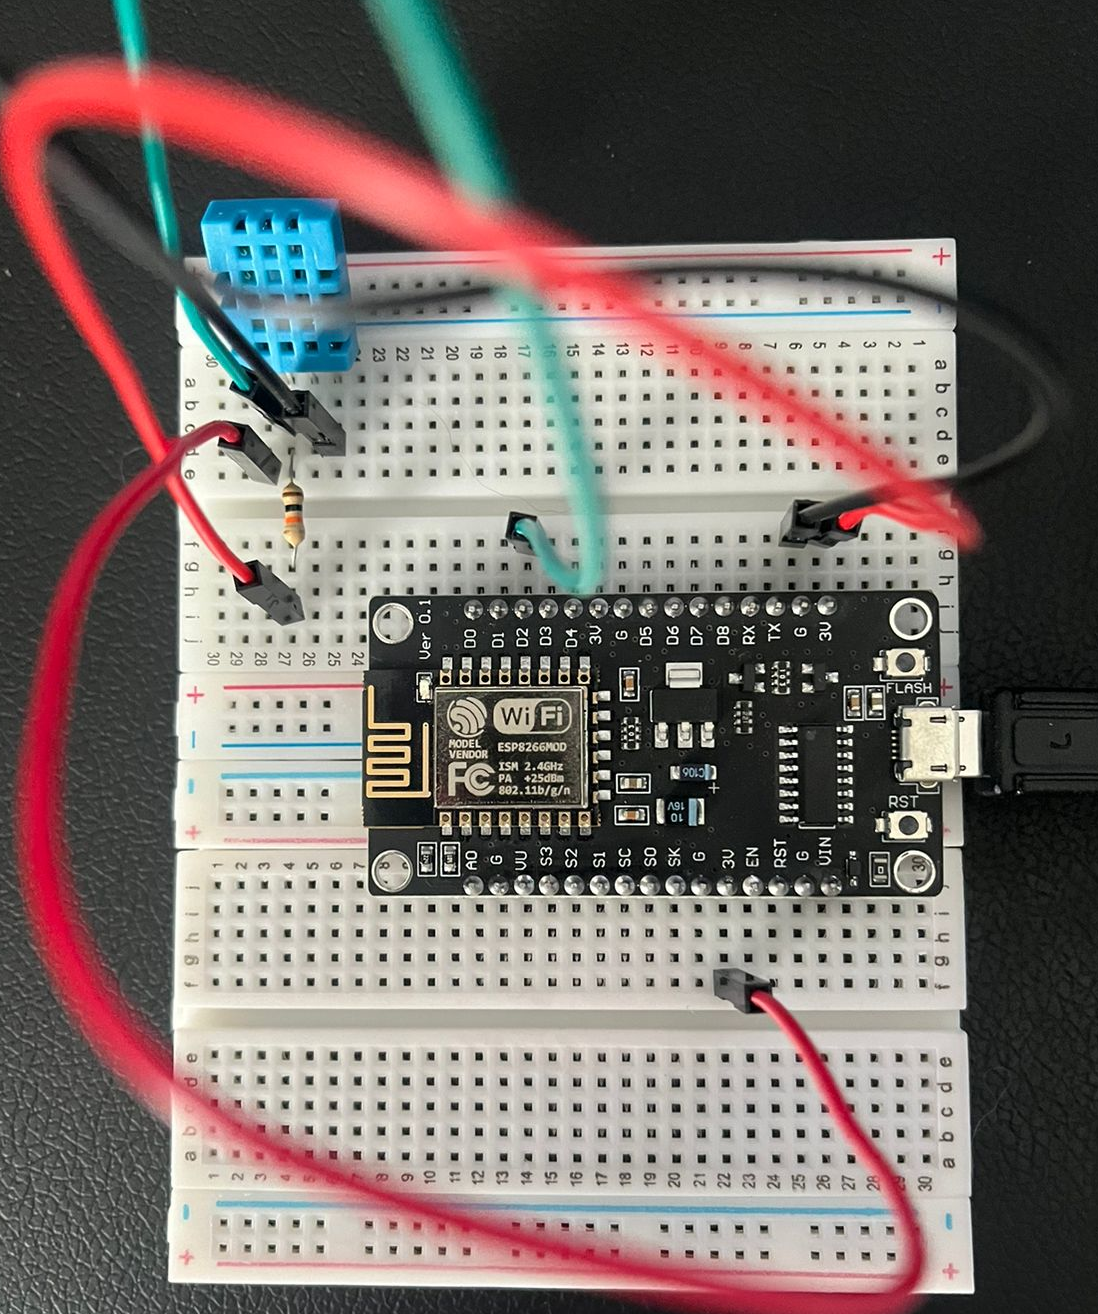
\includegraphics[width=.3\textwidth]{assets/img/project.png}
  \caption{Projeto implementado}
\end{figure}

\section{Ambiente de Desenvolvimento}

Neste capítulo, será detalhado o ambiente de desenvolvimento utilizado, incluindo o sistema operacional, softwares, bibliotecas e os frameworks utilizados para o desenvolvimento e teste do projeto.

\subsection{Sistema Operacional}

O sistema operacional utilizado foi o Debian, uma distribuição Linux, criado em 1993 por Ian Murdock. Ele é um projeto de código aberto mantido por uma comunidade global de desenvolvedores. Esse sistema já era utilizado no ambiente de desenvolvimento em questão, porém, é relevante citar que como o código embarcado desenvolvido, foi escrito usando a linguagem C, é relativamente interessante usar um sistema operacional onde a linguagem C é nativa.

\subsection{ESP8266 RTOS SDK}

O ESP8266 RTOS SDK é um SDK oficial fornecido pela Espressif Systems, projetado especificamente para programar microcontroladores ESP8266. Baseado no sistema operacional FreeRTOS, o SDK oferece uma estrutura para criar as aplicações, gerenciar as bibliotecas, entre outros. Esse SDK também inclui suporte para protocolos mais utilizados em IoT, como: TCP/IP, HTTP/HTTPS e MQTT.

\subsection{Eclipse Mosquitto}

O Eclipse Mosquitto é um broker MQTT leve e de código aberto que facilita a comunicação entre dispositivos IoT. Esse protocolo permite que os dispositivos publiquem e assinem tópicos para a troca de mensagens em tempo real. Nesse projeto, ele foi utilizado apenas para testes, quando o broker remoto não estava disponível.

\subsection{IDE}

O Eclipse IDE for Embedded C/C++ Developers foi a primeira escolha para o desenvolvimento, visto que é uma das plataformas que mais possuem compatibilidade com as diversas bibliotecas disponíveis para o desenvolvimento. Porém, foi observando na documentação que é possível utilizar o Visual Studio Code com a extensão oficial ESP-IDF. Essa extensão fornece todas as funcionalidades que o Eclipse fornece, além de um debugar moderno que permite inclusive monitorar a fila de leituras dos sensores.

\section{Desenvolvimento}

Neste capítulo, será detalhado o que foi planejado e desenvolvido, a fim de atuar como uma possível solução para o problema apresentado anteriormente.

\subsection{Arquitetura da Solução}

\begin{figure}[ht]
  \centering
  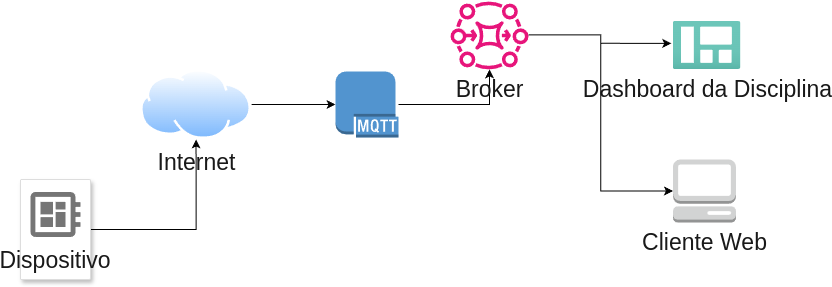
\includegraphics[width=.7\textwidth]{assets/img/architecture.png}
  \caption{Arquitetura do projeto}
\end{figure}

\subsection{Código}

A lógica do código desenvolvido será apresentada a seguir. Inicialmente, é realizada a configuração do armazenamento não volátil (NVS) e a inicialização da conexão Wi-Fi, utilizando um SSID e senha especificados. Foi criado um arquivo separado para não expor as credenciais.

O sensor DHT11 é configurado no pino correspondente, nesse caso o GPIO4. Posteriormente, uma fila dht\_queue é criada para armazenar os dados lidos desse sensor. Além disso, duas tarefas principais são definidas: a tarefa dht\_task, que realiza leituras contínuas do sensor em intervalos de 10 segundos, imprimindo os valores de temperatura e umidade no console e enviando esses dados para a fila.

Da mesma maneira, a tarefa mqtt\_task, aguarda a conexão Wi-Fi, inicializa um cliente MQTT com configurações especificadas, e publica continuamente os dados lidos do sensor nos tópicos MQTT definidos para temperatura e umidade. 

\begin{algorithm}
  \caption{}
  \begin{algorithmic}[1]
  \STATE Inicializar NVS (Non-Volatile Storage)
  \STATE Inicializar Wi-Fi com SSID e senha especificados
  \STATE Inicializar sensor DHT11 no pino definido
  \STATE Criar fila \texttt{dht\_queue} para armazenar dados do sensor DHT
  \STATE Criar tarefa \texttt{dht\_task}:
      \WHILE{verdadeiro}
          \STATE Ler temperatura e umidade do DHT11
          \STATE Imprimir os valores lidos
          \STATE Enviar dados para a fila \texttt{dht\_queue}
          \STATE Aguardar 10 segundos
      \ENDWHILE
  \STATE Criar tarefa \texttt{mqtt\_task}:
      \STATE Aguardar conexão Wi-Fi estabelecida
      \STATE Inicializar cliente MQTT com configurações especificadas
      \WHILE{verdadeiro}
          \STATE Receber dados da fila \texttt{dht\_queue}
          \STATE Publicar temperatura no tópico MQTT definido
          \STATE Publicar umidade no tópico MQTT definido
      \ENDWHILE
  \end{algorithmic}
\end{algorithm}

O código completo pode ser visualizado no seguinte endereço: \url{https://github.com/isabellanunesdev/esp8266-mqtt-temp}

\subsection{Cliente}

Foi desenvolvido um dashboard em React que consome dados de temperatura e umidade a partir do mesmo broker MQTT, que os dados foram enviados. Há também uma feature flag para ativar e desativar o envio de dados para o broker, permitindo assim trocar o broker para um servidor Mosquitto local, que pode ser acessado, rodando o container, descrito no arquivo docker\_compose no repositório do código completo. A ideia desse cliente, é de ter uma página que pode ser acessada na rede local, a fim de visualizar amigavelmente os dados dos sensores.

\begin{figure}[ht]
  \centering
  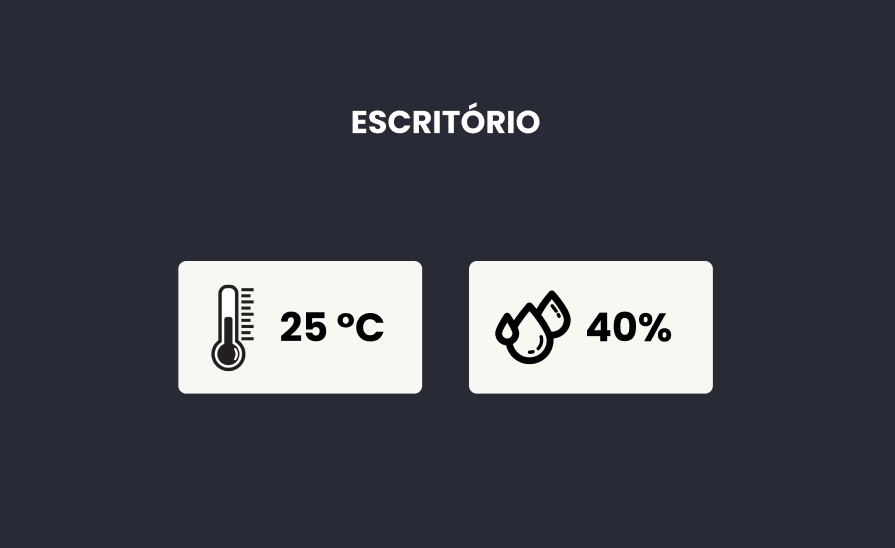
\includegraphics[width=.5\textwidth]{assets/img/client.png}
  \caption{Cliente Web}
\end{figure}

\section{Resultados}

Os resultados apresentados nas imagens a seguir demonstram o funcionamento do sistema IoT desenvolvido. No console do terminal, as leituras do sensor DHT11 são exibidas em tempo real, com valores consistentes de temperatura (23°C) e umidade (50\%), apesar de algumas falhas ocasionais na leitura, indicadas por mensagens de "Timeout" ou "Erro", que estão sendo tratadas.

\begin{figure}[ht]
  \centering
  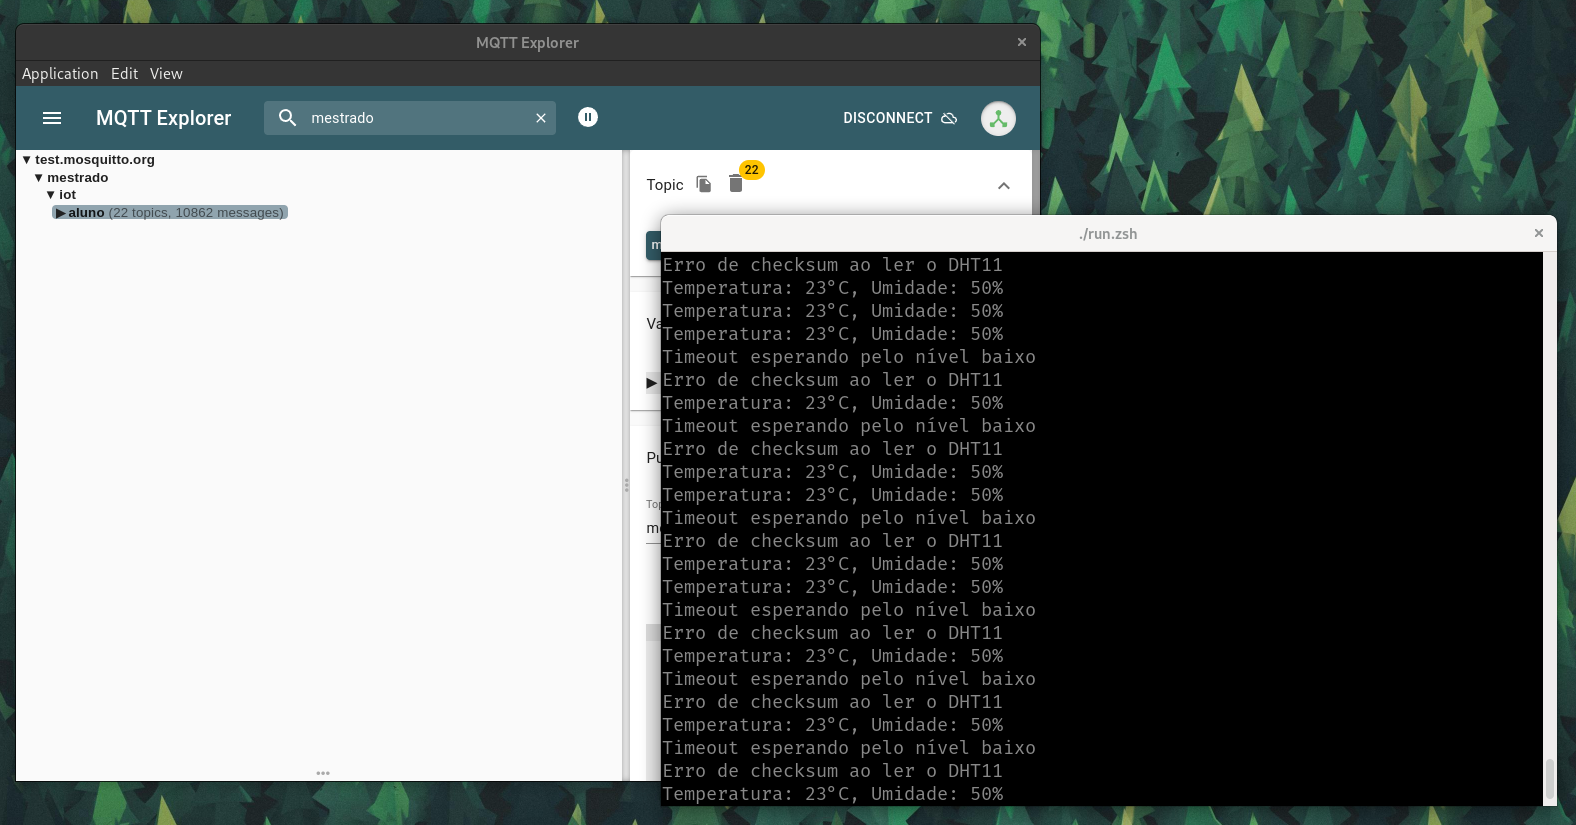
\includegraphics[width=.7\textwidth]{assets/img/results1.png}
  \caption{Projeto rodando}
\end{figure}

No MQTT Explorer, é possível verificar que os dados de temperatura e umidade estão sendo enviados, utilizando os tópicos configurados. Esses resultados demonstram a correta integração entre hardware (ESP8266 e DHT11), software e o protocolo MQTT para transmissão de dados.

\begin{figure}[ht]
  \centering
  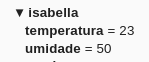
\includegraphics[width=.4\textwidth]{assets/img/results2.png}
  \caption{Dados chegando no broker}
\end{figure}

\section{Conclusão}

Por meio do microcontrolador ESP8266 e do sensor DHT11, foi possível coletar dados de temperatura e umidade e transmiti-los em tempo real via protocolo MQTT. A implementação de um dashboard em React também mostrou como esses dados podem ser consumidos e visualizados localmente, oferecendo um ambiente de visualização amigável, quando o broker não está disponível.

Durante o desenvolvimento, houveram alguns desafios técnicos, como erros ocasionais na leitura do sensor DHT11, concorrência entre as tarefas e dificuldades na configuração do broker MQTT local. Por fim, este relatório demonstrou a possibilidade de desenvolver uma aplicação IoT em um contexto simulado, que se assemelha ao mundo real, a fim de aplicar os conhecimentos adquiridos na disciplina.

\end{document}
